\chapter{Using XML-based Project Configurations}
\label{chap:using-xml-based-project-configurations}

Notice that at this point there are no contents in any of the four tabs.  Opus uses a novel approach to dynamically creating and managing content in the GUI by loading, editing, and saving content in the form of XML files.  XML stands for Extensible Markup Language, and is an extension of the HTML markup language used to display web pages.  It is more flexible, and has become widely used to store content in a strucured form.  

To add content to the GUI, we will load a \emph{Project}, which is in fact, just an XML file containing configuration information.  From the main menu, load a project from eugene\_gridcell.xml, which is in the default location of opus/project\_configs.  The Opus window should now appear as in Figure \ref{fig:opus2}.

\begin{figure}[htp]
\begin{center}
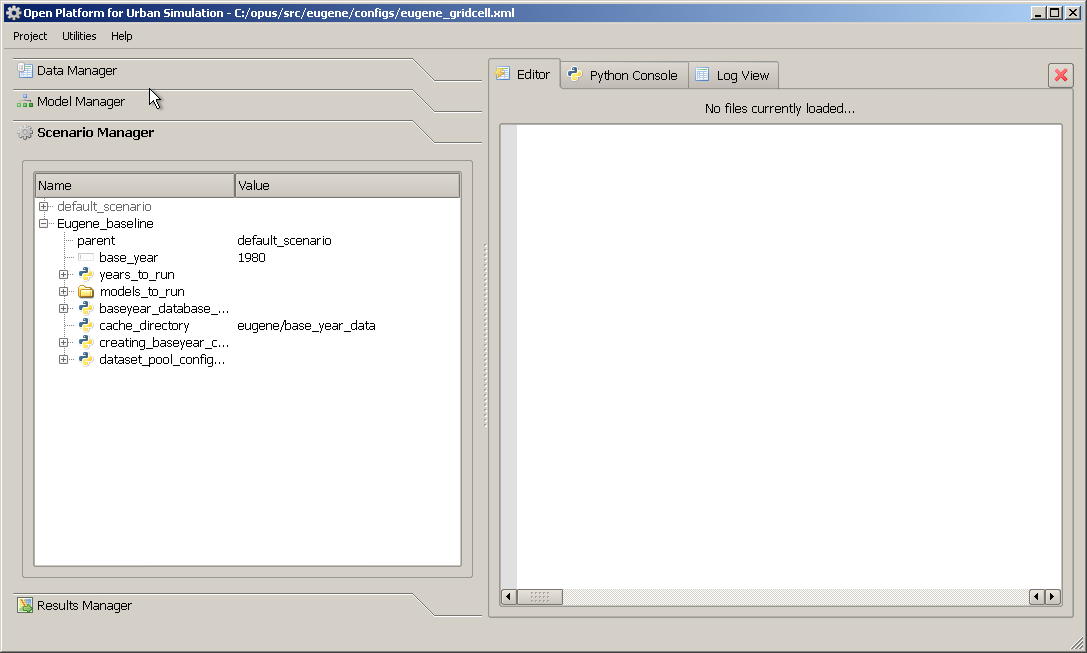
\includegraphics[scale=0.4]{graphics/opus2.png}
\end{center}
\caption{Opus GUI Main Window}
\label{fig:opus2}
\end{figure}

A small section of the eugene\_gridcell.xml file is shown in Figure \ref{fig:opus-xml}.  It is just text, but in a structured format, with nodes corresponding to information that is displayed in the GUI.  Some of the content of the XML provide data used by the GUI to determine how to display information, or what menu items are appropriate to connect to the node in the GUI.

\begin{figure}[htp]
\begin{center}
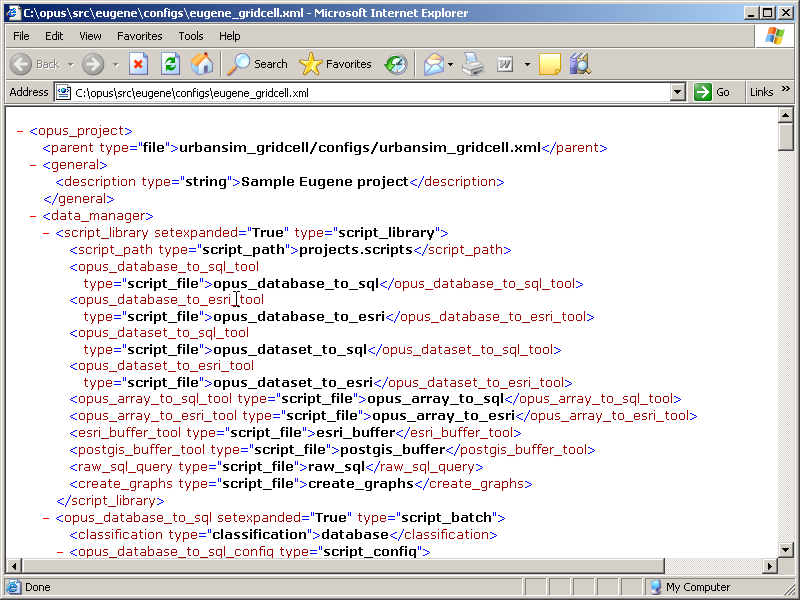
\includegraphics[scale=0.4]{graphics/opus-xml.png}
\end{center}
\caption{An Excerpt from eugene$\_$gridcell.xml}
\label{fig:opus-xml}
\end{figure}

Note that one of the first entries in the xml file is a \emph{parent} type, and that this line refers to another xml file named urbansim/gridcell.xml.  This reflects an important aspect of the GUI design: it supports inheritance among projects.  In practical terms for a user, this means that you can use default projects as templates, or parents, for another project you want to create that is mostly the same as an existing project, but has some changes from it.  The new project is called a \emph{child} project, and it inherits all of its information from the \emph{parent}, but can override any aspect it so chooses from the parent.  The parallels with human behavior are pretty obvious!

Users will create their own projects in the opus/project\_configs directory.  This will allow them to keep projects localized in one place, and to avoid editing and possibly corrupting one of the projects that are in an Opus package.
